\documentclass[border=12pt,tikz]{standalone}
\usepackage{fontspec}
\setmainfont{Helvetica Neue}
\setsansfont{Helvetica Neue}
\setmonofont{Menlo}
\usepackage{tikz}
\usetikzlibrary{positioning, arrows.meta, fit, backgrounds, calc}

\definecolor{l0}{HTML}{E3F2FD}
\definecolor{l0b}{HTML}{90CAF9}
\definecolor{l1}{HTML}{E8F5E9}
\definecolor{l1b}{HTML}{81C784}
\definecolor{l2}{HTML}{FFF3E0}
\definecolor{l2b}{HTML}{FFB74D}
\definecolor{l3}{HTML}{F3E5F5}
\definecolor{l3b}{HTML}{BA68C8}
\definecolor{l4}{HTML}{FCE4EC}
\definecolor{l4b}{HTML}{E57373}
\definecolor{gray50}{HTML}{9E9E9E}

\begin{document}
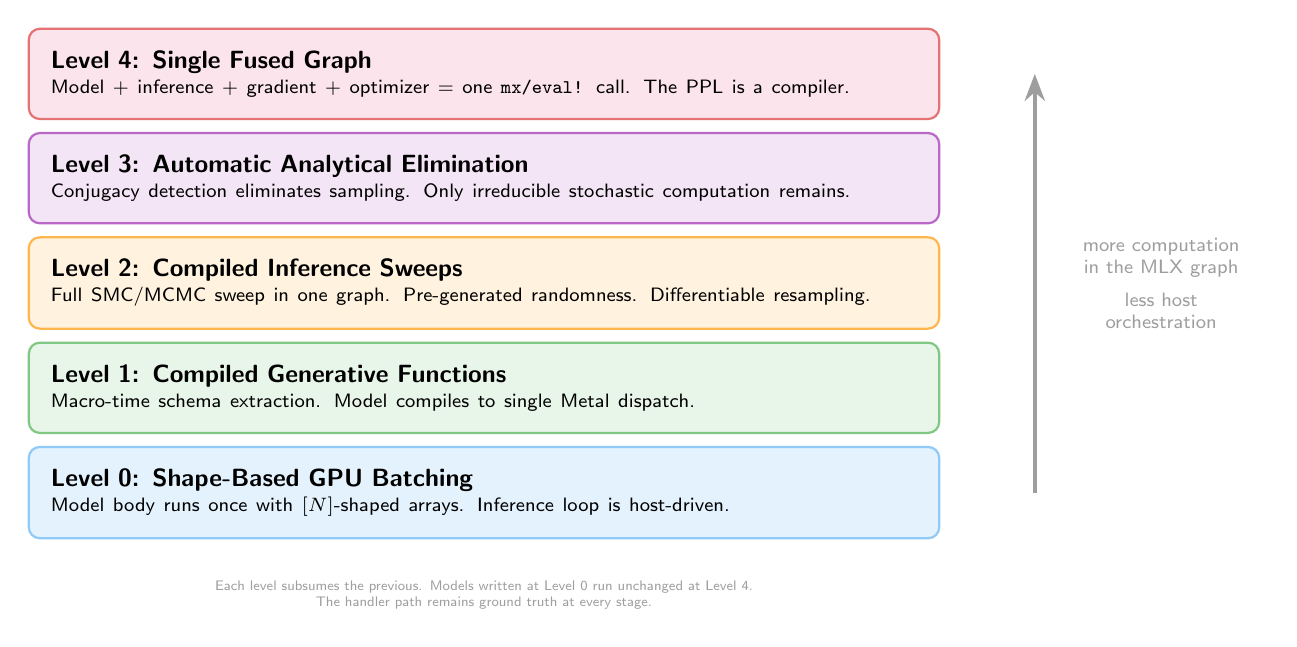
\begin{tikzpicture}[
    >=Stealth,
    node distance=0.15cm,
    level/.style={draw, rounded corners=4pt, minimum height=1.1cm, line width=0.8pt,
                  font=\sffamily\small, align=left, text width=11cm, inner sep=8pt},
    label/.style={font=\sffamily\tiny, color=gray50},
    numlabel/.style={font=\sffamily\footnotesize\bfseries, minimum width=1.2cm, align=center},
]

% Levels (bottom to top, stacking)
\node[level, fill=l0, draw=l0b] (lev0) {
  \textbf{Level 0: Shape-Based GPU Batching}\\[-2pt]
  {\scriptsize Model body runs once with $[N]$-shaped arrays. Inference loop is host-driven.}
};

\node[level, fill=l1, draw=l1b, above=of lev0] (lev1) {
  \textbf{Level 1: Compiled Generative Functions}\\[-2pt]
  {\scriptsize Macro-time schema extraction. Model compiles to single Metal dispatch.}
};

\node[level, fill=l2, draw=l2b, above=of lev1] (lev2) {
  \textbf{Level 2: Compiled Inference Sweeps}\\[-2pt]
  {\scriptsize Full SMC/MCMC sweep in one graph. Pre-generated randomness. Differentiable resampling.}
};

\node[level, fill=l3, draw=l3b, above=of lev2] (lev3) {
  \textbf{Level 3: Automatic Analytical Elimination}\\[-2pt]
  {\scriptsize Conjugacy detection eliminates sampling. Only irreducible stochastic computation remains.}
};

\node[level, fill=l4, draw=l4b, above=of lev3] (lev4) {
  \textbf{Level 4: Single Fused Graph}\\[-2pt]
  {\scriptsize Model + inference + gradient + optimizer = one \texttt{mx/eval!} call. The PPL is a compiler.}
};

% Arrow on the right side
\draw[->, line width=1.5pt, color=gray50]
    ([xshift=1.2cm]lev0.east) -- ([xshift=1.2cm]lev4.east)
    node[midway, right=6pt, font=\sffamily\scriptsize, color=gray50, align=center, text width=2.5cm] {
      more computation\\in the MLX graph\\[4pt]
      less host\\orchestration
    };

% "Each level subsumes the previous" note
\node[label, below=0.4cm of lev0, text width=11cm, align=center] {
  Each level subsumes the previous. Models written at Level 0 run unchanged at Level 4.\\
  The handler path remains ground truth at every stage.
};

\end{tikzpicture}
\end{document}
